\documentclass[11pt]{article}

\usepackage[margin=1.5in]{geometry}

\usepackage{fancyhdr}
\pagestyle{fancy}
\newcommand\course{ASTR 101}
\newcommand\hwnumber{4}
\newcommand\duedate{October 27, 2020}

\lhead{Oliver Tonnesen\\V00885732}
\chead{\textbf{\Large Lab \hwnumber{} Report}}
\rhead{\course\\\duedate}

\usepackage[
	backend=biber,
	url=true
]{biblatex}
\addbibresource{lab4.bib}
\usepackage{enumitem}
\usepackage{graphicx}
\usepackage{url}
\usepackage{pgfplots}
\pgfplotsset{width=10cm,compat=1.9}

\usepackage{multirow}

\usepackage{amsmath,amsfonts,amssymb}


\begin{document}
\section{Objective}
This lab exercise examines the Moon's craters and maria and how they can be studied and used to predict the rate of asteroid impacts with the Earth.


\section{Introduction}
The Moon has always been a significant part of human culture, and its phases are the basis for our $\sim$30 day months.
The Moon is tidally locked with Earth, meaning we always see the same part of the Moon as it orbits us.
The lunar surface has a large number of craters, some of which can even be seen with the naked eye.

Due to its proximity to Earth, the Moon is an important resource for studying the evolution of other planets and moons, and the history of meteor impacts in the Solar System.
In this lab, we see an example of this by estimating the rate at which Earth is impacted by large meteors by studying the craters on the Moon.


\section{Procedure}
\subsection*{Part 1: Lunar feature identification}
Using a high resolution image of the Moon, an online lunar map~\cite{moon-map}, and GIMP, we observed the lunar surface and mapped out some significant craters, maria, and spacecraft landing sites.


\subsection*{Part 2: Meteorite size and crater size}
We started by determining a scale factor to convert between distance in pixels in our image and distance in kilometres.
Using the rule of thumb that the diameter of a crater is between 10 to 50 times the diameter of the meteorite that created it, we estimated the size of the meteorites that created various craters on the Moon.
We then searched the lunar surface for craters similar in size to various craters on the Earth.


\subsection*{Part 3: Impact effects}
We used an online tool~\cite{impact-simulator} to simulate the effects of impacts with asteroids with varying sizes and densities.


\subsection*{Part 4: Large impact rate estimation}
We started by counting the number of craters on the lunar surface.
We used this number along with the ratio between the surface area of the Earth and the Moon to estimate how frequently the Earth is impacted by asteroids of significant size (at least 1 km in diameter).


\section{Observations, Tables, and Graphs}
\begin{figure}[h]
\begin{center}
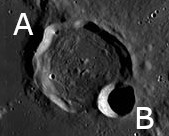
\includegraphics[width=0.75\columnwidth]{figures/overlapping_craters.jpg}
\end{center}
\caption{Two overlapping lunar craters.}
\label{img:overlapping-craters}
\end{figure}


\section{Answers}
\begin{enumerate}[label={\textbf{\emph{(\arabic*)}}}]
	\item % 1
Please see the lunar image provided in the attached PDF, lunar\_surface.pdf.
We list the labelled craters, maria, and spacecraft landing sites:
\begin{itemize}
\item Grimaldi crater
\item Plato crater
\item Tycho crater
\item Mare Imbrium
\item Mare Serenitatis
\item Mare Tranquilitatis
\item Apollo 11
\item Apollo 14
\item Apollo 17
\end{itemize}

	\item % 2
We see that the crater labelled B in Figure~\ref{img:overlapping-craters} dominates the crater labelled A, so we can conclude that A formed first, and B formed after.

	\item % 3
In a crater formed more recently than a mare, we expect to see lighter coloured rock both in the crater, and scattered around it.
These features can all be seen in the Copernicus crater (labelled in lunar\_surface.pdf).
Conversely, we expect to see none of these features in a crater formed before a mare.
The Archimedes crater (labelled in lunar\_surface.pdf) looks almost as though it is a part of the Mare Imbrium, only that it is surrounded by a rim and lacks the rays of ejected material characteristic of younger impact craters.

	\item % 4
The Kepler and Copernicus craters labelled in lunar\_surface.pdf are two examples of craters from which protrude with lighter coloured rays of ejected material.

	\item % 5
The diameter of the image of the moon is 10 000 px, so the scale of our image in km/px is 3476 km/10 000 px = 0.347 6 km/px.

	\item % 6
We choose Archimedes to be our large crater, and the crater just to the left of Kepler to be our small crater.
These craters have size 229 px and 15.0 px, respectively.
Using our scale of 0.347 6 km/px, this gives us actual sizes of 79.6 km and 5.21 km, respectively.

	\item % 7
The meteorite that created the large crater should have been between 79.6 km/50 = 1.6 km and 79.6 km/10 = 8.0 km, and the meteorite that created the small crater should have been between 5.21 km/50 = 0.10 km and 5.21 km/10 = 0.52 km.

	\item % 8
Using our scale of 0.347 6 km/px, we want to find craters of size approximately 1.2 km/0.347 6 km/px = 3.4 px, 100 km/0.347 6 km/px = 288 px, and 180 km/0.347 6 km/px = 518 px.
These craters are labelled as A, B, and C (from smallest to largest) in the same image that was used in part 1.

	\item % 9
Assuming 99942 Apophis is fairly dense (3000 kg/m$^3$) and impacts sedimentary rock, the crater would have a diameter of around 4.2 km, and a depth of almost 0.5 km.
Assuming comet Swift-Tuttle has density 1000 kg/m$^3$ and impacts sedimentary rock, the crater would have a diameter of almost 300 km, and would be over 1.5 km deep.

	\item % 10
99942 Apophis is an asteroid, thus made of relatively dense rock.
3000 kg/m$^3$ is roughly half the density of iron, so it seems like a decent estimate of the asteroid's density.
Swift-Tuttle is a comet, so it's made primarily of ice which has a density of 900 kg/m$^3$; we rounded up to 1000 kg/m$^3$ to account for any denser components that may comprise the comet.
Sedimentary rock covers over 80 percent of the surface of the Earth~\cite{britannica-sedimentary}, so it's not unlikely that a meteorite might hit sedimentary rock if it were to impact Earth.

	\item % 11
In the case of an impact from Apophis in water of depth 30 m, the resulting tsunami 300 km away would be 28.5 cm high, and if Swift-Tuttle were to impact Earth with the same parameters, the resulting tsunami would be 12 m high.

	\item % 12
If Apophis were to impact the Earth, we would be relatively safe at a distance of 300 km.
It would be a much different story if we were to be impacted by Swift-Tuttle: while at 300 km away we might possibly escape the effects of the tsunami, we would definitely feel the effects of the fireball caused by the impact, and also the 4000 m/s winds.

	\item % 13
If a 1 km asteroid with density 3000 kg/m$^3$ and velocity 20 m/s were to hit sedimentary rock, then the resulting crater would have a diameter of about 16 km, and a depth of almost 700 m.

	\item % 14
It appears as though more craters formed early on in this history of the Solar System.
One reason this may be the case is because there was much more debris flying around when the Solar System was young and the planets were still forming.
If the giant impact hypothesis is true, and the Earth was struck with an ancient planet that became then moon, then there certainly must have been an enormous amount of debris that was constantly impacting the moon.
The impacts from this debris would have slowed over time, explaining why there seem to be far fewer recent impacts than early impacts.

	\item % 15
We counted 120 $\pm$ 9 asteroids of diameter at least 1 km on the maria.
120 $\pm$ 9 asteroids/0.16 = 750 $\pm$ 56 asteroids of diameter at least 1 km.
This calculation assumes that asteroids impact the surface of the moon uniformly.

	\item % 16
3.5 billion years/(750 $\pm$ 56 asteroids of diameter at least 1 km) = 4.6 $\pm$ 0.3 million years / (asteroid of diameter at least 1 km).

	\item % 17
$\frac{1}{4.6 \pm 0.3 \textrm{million years / (asteroid of diameter at least 1 km)}}$ = $(2.2 \pm 0.15) \times 10^{-7}$ asteroids of diameter at least 1 km / year.

	\item % 18
The Earth's surface area is approximately 13.4 times that of the Moon.
$13.4 \cdot (2.2 \pm 0.15) \times 10^{-7} = (3 \pm 0.2) \times 10^{-6}$ asteroids of diameter at least 1 km / year.
This calculation assumes that any point on the Earth is equally likely to be impacted as any point on the Moon.

	\item % 19
It may be possible that the Earth is more likely to be hit than the Moon, since its much higher mass may pull asteroids towards it more.
On the other hand, the Moon may act as a ``shield'', and take more asteroid impacts due to its orbit around the Earth (this seems unlikely, however, due to the Moon's distance from Earth).
		
	\item % 20
In question \textbf{\emph{(18)}} we estimated that significant asteroid impacts occur at a rate of approximately $3 \times 10^{-6}$ impacts per year.
The inverse of this is 330 000 years per impact.
The earliest fossil evidence of Homo sapiens is from around 300 000 years ago, with modern societal behaviour exhibited as early as 70 000 years ago.
This means that -- depending on how one defines "human civilization" -- the average period between significant asteroid impacts is close to the age of human civilization.

	\item % 21
The main reason for the lack of craters on Earth is its atmosphere.
The large majority of asteroids that would impact Earth disintegrate in its atmosphere before they make it to the ground.
This is not the case on the Moon, where even the smallest of debris will likely make it to the ground and create a crater.
Another reason for the disparity in number of craters between Earth and the Moon is that the Earth has water and is tectonically active, meaning even if it is impacted, its craters can erode over time.
This is also not the case on the moon, where craters are basically permanent unless they get buried underneath an even larger crater.

\end{enumerate}


\section{Discussion}
This lab exercise demonstrated how to study and measure craters on the lunar surface.
We learned how to use data from these measurements to estimate the rate of asteroid impacts with Earth.


\subsection*{Part 2: Meteorite size and crater size}
In this section of the lab, we used the known diameter of the Moon to convert between distance in pixels in the image and distance in kilometres.
The photograph is very high resolution, so the scale of 0.347 6 km/px is probably very accurate.

Some sources of uncertainty in this section are error in measuring the pixel distances in the image, and not accounting for the angle at which a crater is facing us on the lunar surface, potentially causing us to measure it to be smaller than it really is.


\subsection*{Part 3: Impact effects}
In this section of the lab, we used the impact simulator provided at~\cite{impact-simulator} to simulate collisions between Earth and two near-Earth objects.
For question \textbf{\emph{(13)}}, we assumed a density of 3000 kg/m$^3$, a speed of 20 m/s, and an impact target of sedimentary rock.

The densest meteorites to hit Earth would likely contain lots of iron, which has a density of around 7.87 g/cm$^3$ = 7870 kg/m$^3$, and the least dense meteorites to hit Earth would likely contain lots of ice, which has a density of around 0.917 g/cm$^3$ = 917 kg/m$^3$.
We assumed iron-rich asteroids to be more rare than comets made primarily of ice, so we chose our density of 3000 kg/m$^3$ to be just less than halfway between these two extremes.

According to NASA~\cite{nasa-impact}, an average asteroid travels at 20 m/s, so we used this value in our simulation.

Over 80 percent of the surface of the Earth is covered by sedimentary rock~\cite{britannica-sedimentary}, so we chose it to be our asteroid's impact target in the simulation.


\subsection*{Part 4: Large impact rate estimation}
In this section of the lab, we counted the number of craters on the maria caused by asteroids with diameter at least 1 km.

We counted 120 craters that were definitely created by a asteroid larger than 1 km, and 9 craters that were very close, and could have been created by a asteroid either smaller or larger than 1 km.
This process of counting craters is quite error-prone, and was definitely a source of significant uncertainty.
To account for this, we use the 9 craters that were very close in size as our uncertainty.


\section{Conclusion}
In this lab exercise, we learned about the observation, measurement, and study of lunar craters and how they can be used to to estimate the rate at which Earth is impacted by large asteroids.
We also ran some simulations to see what impacts with such asteroids would look like from our perspective on Earth.


\printbibliography


\end{document}
